% ICASSP 2026 short-paper draft distilled from main5.tex (single-stream path only).
% Replace the placeholder author and affiliation fields before submission.
\documentclass{article}
\usepackage{spconf,amsmath,amssymb,graphicx,booktabs,multirow}
\usepackage{placeins,float}
\usepackage{cite}
\usepackage{url}
\newcommand{\metrictriplet}[3]{\makebox[3.1em][c]{#1}\hspace{0.5em}\makebox[3.1em][c]{#2}\hspace{0.5em}\makebox[3.1em][c]{#3}}
\newcommand{\metricheader}{\makebox[3.1em][c]{AP}\hspace{0.5em}\makebox[3.1em][c]{AP$_{50}$}\hspace{0.5em}\makebox[3.1em][c]{AP$_{75}$}}
\newcommand{\citerange}[2]{\mbox{\cite{#1}\textendash\kern-0.38em\cite{#2}}}

\title{PROMPTMINER-SAM2: PROMPT MINING and Uncertainty-Guided Refinement FOR REMOTE SENSING INSTANCE SEGMENTATION}
\name{Anonymous Author(s)}
\address{Anonymous Affiliation(s)}

\begin{document}
\maketitle

\begin{abstract}
Existing remote sensing instance segmentation methods predict masks using implicit instance representations. 
Although they can encode instance semantics, they lack explicit constraints on local shapes, which can lead to boundary ambiguities in complex backgrounds and between adjacent instances.
To address this limitation, we propose PromptMiner-SAM2, a SAM2-based automatic prompting framework for remote-sensing instance segmentation that explicitly converts the local shapes of candidate regions into mask decoding conditions.
Specifically, the coarse shape prompt mining module (CSPM) predicts the local coarse shapes from candidate region-level features and generates shape-aware prompts accordingly; 
On this basis, a decoder-tail module (UDR) is designed to identify uncertain pixels and correct their predictions using local mask features and instance context.
Experiments on the WHU and NWPU VHR-10 benchmarks show that PromptMiner-SAM2 achieves
mask AP values of 73.4\% and 68.3\%, respectively, attaining the highest mask AP among the compared
methods.
\end{abstract}
\begin{keywords}
Instance segmentation, remote sensing imagery, SAM2, prompt mining, mask refinement
\end{keywords}

\section{INTRODUCTION}

Remote-sensing instance segmentation predicts a pixel-level mask for each object, supporting urban planning and disaster assessment~\cite{rsiisn},~\cite{p2pformer}.
High-resolution remote-sensing images often exhibit scale variation and complex background textures.
These factors make local target--background and inter-instance boundaries difficult to distinguish, hindering accurate mask prediction.

Existing methods use two-stage, one-stage, conditional, or set-prediction paradigms and represent objects with candidate-region features, dynamic parameters, or instance queries to predict masks~\citerange{maskrcnn}{condinst},~\cite{mask2former}.
For remote-sensing imagery, prior work improves mask prediction through multi-scale feature fusion, boundary modeling, and foundation-model adaptation~\cite{rsiisn},~\cite{p2pformer},~\cite{rs4d},~\cite{directsamrs}. 
Automatic prompt learning and detector-to-SAM prompt transfer further extend prompt-based remote-sensing segmentation~\citerange{sam}{pasam},~\cite{rsprompter},~\cite{airwaysam}.

Despite their different formulations, most methods predict masks directly from implicit instance representations. 
Local shape information therefore remains entangled with semantic representations and cannot serve as an independent spatial condition in mask decoding.
Existing mask optimization work shows that  that explicit spatial prompts can optimize existing masks.~\cite{samrefiner}.
This paper investigates learning a local coarse shape from candidate-region features and mining it into shape-aware prompts that provide an independent spatial condition for prompt-based instance-mask prediction.


\begin{figure}[t]
\centering
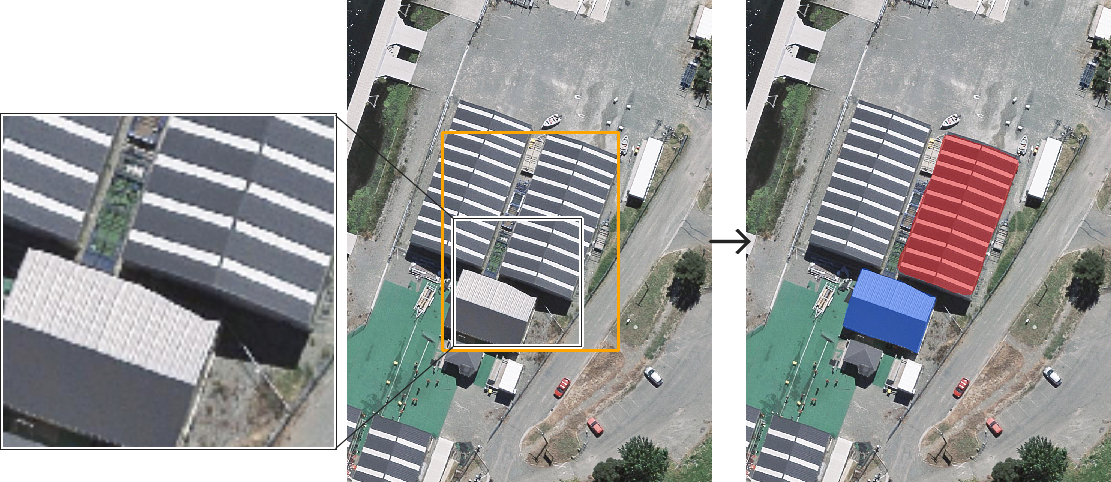
\includegraphics[width=\columnwidth]{teaser_300838_minimal_zoom.png}\par
\vspace{-0.15em}
{\small
\makebox[.5\columnwidth][c]{(a)}%
\makebox[.5\columnwidth][c]{(b)}\par}
\vspace{-0.3em}
\caption{Motivation for instance-local shape. (a) A candidate box specifies the spatial extent of adjacent buildings but does not explicitly provide a local shape condition for mask decoding (zoomed view). (b) Ground-truth instance masks reveal the local shape and boundary information needed to distinguish adjacent instances.}
\label{fig:motivation}
\end{figure}

\begin{figure*}[!t]
\centering
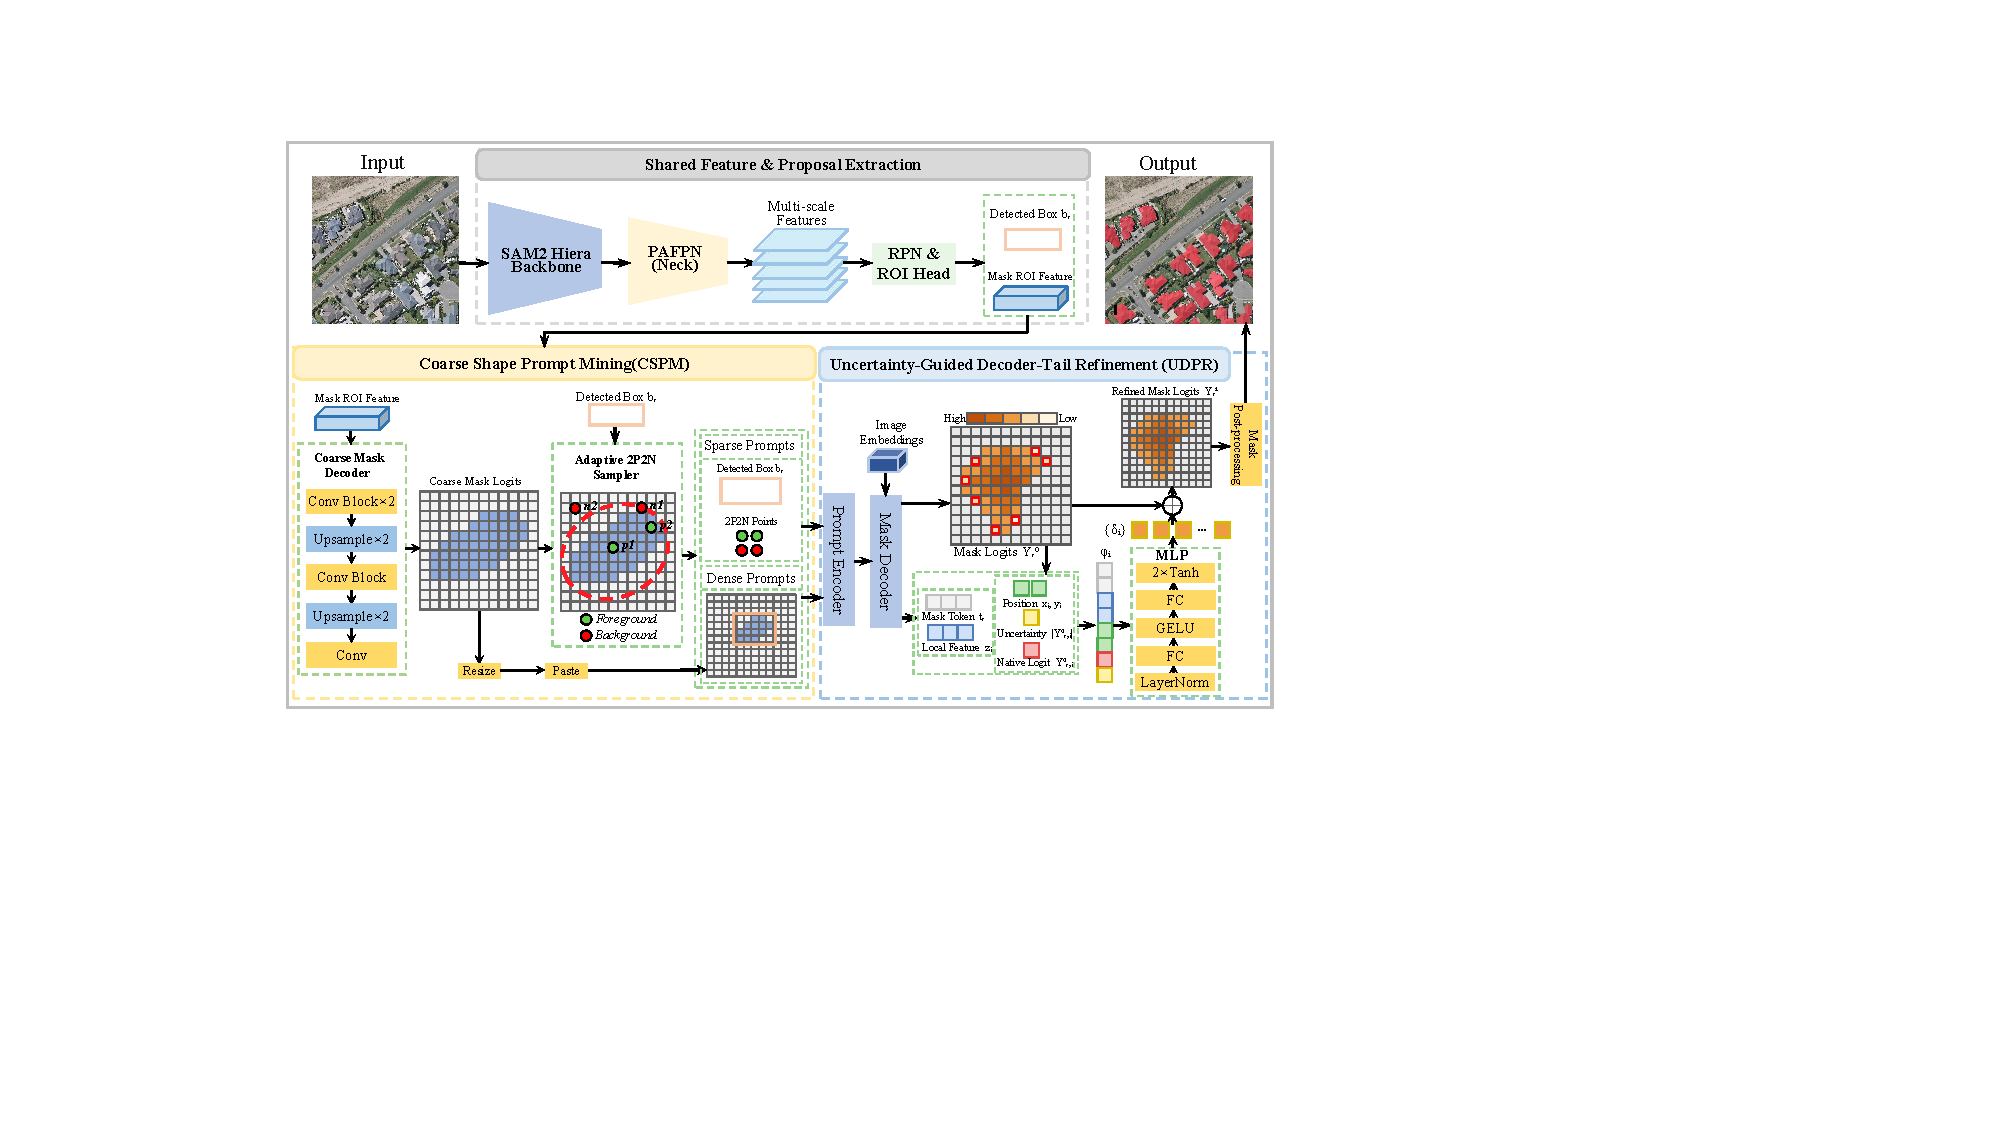
\includegraphics[width=\textwidth]{总体架构图.pdf}
\caption{Overview of PromptMiner-SAM2. The diagram shows the main data flow from the input image and candidate-region features through SAM2 mask decoding to final instance masks. CSPM mines local shape conditions and generates automatic prompts, whereas UDR selectively corrects uncertain regions in the initial masks.}
\label{fig:arch}
\end{figure*}

To address this question, PromptMiner-SAM2 learns a local coarse shape from candidate-region features as an intermediate representation and mines shape-aware prompts from it to provide an independent spatial condition for mask decoding. Figure~\ref{fig:arch} presents the overall framework.

To summarize, our contributions are as follows:
\begin{itemize}
  \item We propose PromptMiner-SAM2, a SAM2-based automatic prompting framework that combines a two-stage detector with the SAM2 prompt-based mask decoder and automatically constructs candidate-region-conditioned decoding prompts.
  \item We design CSPM and UDR. CSPM learns a candidate-region-local coarse shape and mines shape-aware prompts from it, whereas UDR selectively corrects uncertain locations in the initial masks.
  \item We evaluate PromptMiner-SAM2 on the WHU and NWPU VHR-10 remote-sensing benchmarks and systematically analyze the effects of prompt combinations and UDR on instance localization and mask prediction. The complete framework achieves the highest mask AP among the compared methods, while the ablations quantify the complementary roles of sparse prompts, dense shape conditions, and local uncertainty correction.
\end{itemize}

\section{METHOD}
\subsection{Overall Architecture}
As shown in Fig.~\ref{fig:arch}, PromptMiner-SAM2 combines a two-stage detector with the SAM2 prompt-based mask decoder, forming a unified pipeline from instance localization to mask prediction.
For an input image, the SAM2 Hiera image encoder first extracts multi-scale features. The detection branch produces candidate-region features and their spatial extents through the PAFPN, RPN, and RoI pathways, while Hiera features also provide image embeddings for SAM2 mask decoding.
CSPM mines automatic prompts from the candidate-region features. SAM2 decodes these prompts together with the image embedding into initial instance masks, and UDR selectively corrects uncertain local regions to obtain the final masks.

\subsection{Coarse-Shape Prompt Mining}
CSPM learns a local coarse shape from candidate-region features and mines shape-aware prompts from it for SAM2 mask decoding. Let $r$ denote a candidate region with RoI feature $X_r$ and corresponding detection box $b_r$. Here, $X_r$ encodes local visual and shape information within the candidate region, whereas $b_r$ specifies its spatial extent and coordinate reference. The mined prompts include sparse point prompts and a dense shape prompt.

\indent First, the coarse-shape branch maps $X_r$ to a shape logit map defined in the candidate-box-local coordinate system:
\begin{equation}
C_r=f_{\mathrm{coarse}}(X_r),\qquad C_r\in\mathbb{R}^{1\times64\times64}.
\label{eq:coarse}
\end{equation}
\indent During training, the ground-truth instance mask is cropped by the candidate box and mapped to the same local coordinate system to supervise coarse-shape learning. Its independent loss guides $C_r$ to learn the foreground layout and boundary structure within the candidate region.

\indent We then convert the coarse-shape logits into foreground probabilities by $p_r=\sigma(C_r)$ and determine the foreground support with a probability threshold of $0.5$. For a pixel location $u$ on the local shape map, $\bar d_r(u)$ denotes its internal distance to the predicted foreground boundary, normalized by the shorter side of the local shape map. Two positive points are selected sequentially from pixels satisfying foreground-confidence and internal-distance constraints, using $p_r(u)\bar d_r(u)$ as the score; the second positive point additionally avoids a predefined neighborhood around the first. Two negative points are selected sequentially from a one-pixel-wide low-probability outer ring and low-probability background outside the dilated foreground, using $1-p_r(u)$ as the score; the second negative point also avoids the first positive and first negative points.

\indent The box $b_r$ serves as the common spatial reference for the three prompt types. The selected local points are mapped to image coordinates and, together with their positive or negative labels, form the sparse prompt set $\mathcal{S}_r$. The local coarse-shape logits are resized and placed in the image region covered by $b_r$ to form the dense prompt $Q_r$, while $b_r$ itself is used as the box prompt. SAM2 jointly decodes the three prompts with the image embedding:
\begin{equation}
Y_r^0=\mathcal{D}\bigl(\mathcal{E}_I(I),
\widetilde{\mathcal{E}}_P(\mathcal{S}_r,b_r,Q_r)\bigr),
\label{eq:native-decoding}
\end{equation}
\indent where $\mathcal{E}_I$, $\widetilde{\mathcal{E}}_P$, and $\mathcal{D}$ denote the image encoder, prompt-embedding pathway, and mask decoder, respectively. Formed from signed coarse-shape logits, $Q_r$ preserves continuous foreground/background confidence information.

\subsection{Uncertainty-Guided Decoder-Tail Refinement}
UDR corrects the lowest-confidence local locations in the initial SAM2 instance-mask prediction. A single prompt-based decoding pass produces the initial logit map $Y_r^0$, the spatially aligned decoder feature map $U_r$, and the instance-related mask token $t_r$. UDR predicts local residuals only at selected locations, leaving the original decoder output unchanged elsewhere.

\indent UDR first locates uncertain regions on the decoder output grid $\mathcal{G}_r$ of the initial logit map $Y_r^0$. Locations with smaller logit magnitudes lie closer to the foreground/background decision boundary and are therefore more uncertain. We select the $K_r$ most uncertain locations as follows:
\begin{equation}
\begin{aligned}
K_r&=\min(K,|\mathcal{G}_r|),\\
\Omega_r&=\operatorname{BottomK}\bigl(|Y_r^0|,K_r\bigr),\qquad K=64,
\end{aligned}
\label{eq:udpr-selection}
\end{equation}
\indent Here, $\operatorname{BottomK}$ returns the $K_r$ indices in $\mathcal{G}_r$ with the smallest logit magnitudes.

\indent For each selected location $i\in\Omega_r$, we extract a local feature $z_i$ from the aligned feature map $U_r$ and concatenate it with the instance token, normalized coordinates, corresponding logit, and logit magnitude:
\begin{equation}
\phi_i=[z_i,t_r,Y^0_{r,i},x_i,y_i,|Y^0_{r,i}|].
\label{eq:udpr-input}
\end{equation}
\indent Here, $x_i$ and $y_i$ are the normalized horizontal and vertical coordinates of $i$ in $\mathcal{G}_r$. This feature combines local decoding evidence, instance-level context, and the current prediction state, enabling residual prediction to adapt to each instance and location. A lightweight MLP $g$ then predicts a bounded residual for each selected location; mask supervision guides the residual toward the correct foreground or background state:
\begin{equation}
\delta_i=2\tanh g(\phi_i),\qquad i\in\Omega_r,
\label{eq:udpr}
\end{equation}

\indent Finally, the predicted residuals are written back to their corresponding locations to form the refined logit map:
\begin{equation}
Y^1_{r,i}=\begin{cases}
Y^0_{r,i}+\delta_i, & i\in\Omega_r,\\
Y^0_{r,i}, & i\notin\Omega_r.
\end{cases}
\label{eq:udpr-scatter}
\end{equation}
\indent This selective update corrects only locations in $\Omega_r$ and leaves all remaining decoder outputs unchanged, thereby applying bounded local residual correction on the existing SAM2 decoder output grid.

\section{EXPERIMENTS}
\subsection{Experimental Setup}
We evaluate the method on two remote-sensing benchmarks, WHU and NWPU VHR-10. WHU is a single-class building instance segmentation benchmark with 2,943/627/2,220 training, validation, and test images~\cite{whu}. NWPU VHR-10 is a ten-class object detection benchmark~\cite{nwpu}; because its original release provides detection annotations only, we use the publicly released instance masks of Su \textit{et al.}~\cite{nwpu_instance} and their 520/130 train/evaluation split.

We implement the model in PyTorch and train it with distributed data parallelism on four NVIDIA RTX 3090 GPUs. Each GPU processes one image, and two-step gradient accumulation yields an effective batch size of eight. Both benchmarks are initialized from SAM2 Hiera-Base+ weights: the Hiera backbone remains frozen, while its adaptation modules, the prompt pathway, and the mask decoder are trained. We use AdamW with an initial learning rate of $5\times10^{-4}$ and cosine annealing; the training objective jointly includes detection, coarse-shape prompting, and final instance-mask losses.

Under a common development protocol, we select UDR correction locations from $K\in\{32,64,128\}$. Table~\ref{tab:k-sensitivity} shows that $K=64$ achieves the highest overall bbox AP and mask AP; we therefore use it in the main experiments.

\begin{table}[!t]
\caption{Sensitivity of $K$ on the NWPU VHR-10 dataset under a common development protocol.}
\label{tab:k-sensitivity}
\centering
\small
\begin{tabular}{c ccc ccc}
\toprule
& \multicolumn{3}{c}{Bbox (\%)} & \multicolumn{3}{c}{Mask (\%)} \\
\cmidrule(lr){2-4}\cmidrule(lr){5-7}
$K$ & AP & AP$_{50}$ & AP$_{75}$ & AP & AP$_{50}$ & AP$_{75}$ \\
\midrule
32  & 69.38 & 91.69 & 79.03 & 64.94 & 92.91 & 70.01 \\
64  & \textbf{70.35} & 92.23 & \textbf{81.65} & \textbf{66.65} & \textbf{94.15} & 71.97 \\
128 & 70.13 & \textbf{92.42} & 81.32 & 65.97 & 93.71 & \textbf{72.22} \\
\bottomrule
\end{tabular}
\end{table}

\subsection{Comparative Analysis}
We compare PromptMiner-SAM2 with 10 representative instance segmentation methods. For analysis, the compared methods are grouped into CNN-based methods (CNN) and global sequence modeling methods (GSM). The former includes two-stage, one-stage, and cascade designs, whereas the latter includes Transformer-style mask prediction and foundation-model prompting. The \emph{Type} column in Table~\ref{tab:comparison} uses these abbreviations.

\begin{figure*}[t]
\centering
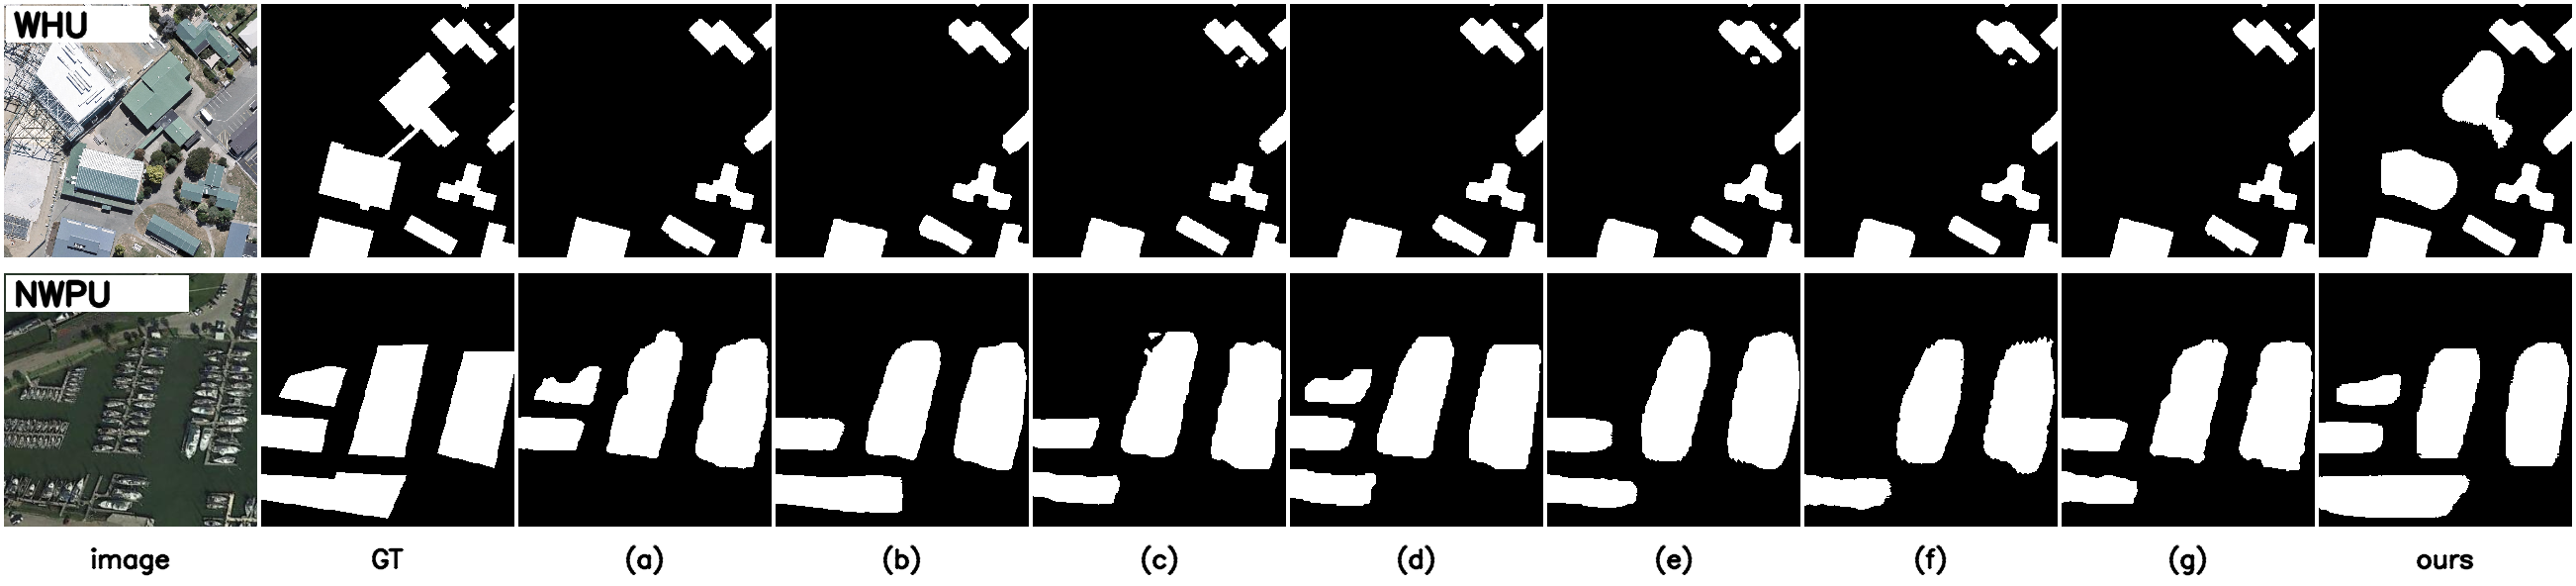
\includegraphics[width=\textwidth]{viz_grid_row_combined.png}\par
\vspace{-0.15em}
{\small
\makebox[.1\textwidth][c]{Input}%
\makebox[.1\textwidth][c]{GT}%
\makebox[.1\textwidth][c]{(a)}%
\makebox[.1\textwidth][c]{(b)}%
\makebox[.1\textwidth][c]{(c)}%
\makebox[.1\textwidth][c]{(d)}%
\makebox[.1\textwidth][c]{(e)}%
\makebox[.1\textwidth][c]{(f)}%
\makebox[.1\textwidth][c]{(g)}%
\makebox[.1\textwidth][c]{Ours}\par}
\vspace{-0.3em}
\caption{Qualitative comparison on WHU and NWPU VHR-10. From left to right, the columns show the input image, ground truth, and predictions of (a) MaskDINO, (b) RSPrompter, (c) CondInst, (d) YOLO11, (e) HTC, (f) Mask R-CNN, (g) M2F, and PromptMiner-SAM2 (ours).}
\label{fig:qualitative}
\end{figure*}

\begin{table*}[t]
\caption{Comparative analysis on the WHU dataset and the NWPU VHR-10 dataset. Each entry reports AP / AP$_{50}$ / AP$_{75}$ (\%) for the Bbox and Mask columns.}
\label{tab:comparison}
\centering
\small
\begingroup
\setlength{\tabcolsep}{3pt}
\renewcommand{\arraystretch}{1.08}
\begin{tabular}{llcccc}
\toprule
& & \multicolumn{2}{c}{WHU} & \multicolumn{2}{c}{NWPU VHR-10} \\
\cmidrule(lr){3-4}\cmidrule(lr){5-6}
& & Bbox (\%) & Mask (\%) & Bbox (\%) & Mask (\%) \\
\cmidrule(lr){3-3}\cmidrule(lr){4-4}\cmidrule(lr){5-5}\cmidrule(lr){6-6}
Type & Method & \metricheader & \metricheader & \metricheader & \metricheader \\
\midrule
\multirow{5}{*}{\textit{CNN}} & Mask R-CNN~\cite{maskrcnn} & \metrictriplet{70.9}{89.9}{80.9} & \metrictriplet{68.2}{90.0}{80.0} & \metrictriplet{65.4}{90.2}{78.9} & \metrictriplet{63.0}{90.1}{71.2} \\
& MS R-CNN~\cite{msrcnn} & \metrictriplet{68.8}{89.4}{80.0} & \metrictriplet{67.7}{89.6}{79.5} & \metrictriplet{67.8}{94.3}{83.8} & \metrictriplet{64.7}{93.6}{\textbf{80.8}} \\
& HTC~\cite{htc} & \metrictriplet{72.7}{90.6}{82.5} & \metrictriplet{69.2}{90.7}{81.6} & \metrictriplet{58.9}{86.9}{67.7} & \metrictriplet{51.3}{84.6}{53.3} \\
& CondInst~\cite{condinst} & \metrictriplet{74.2}{90.0}{82.4} & \metrictriplet{69.7}{90.2}{80.9} & \metrictriplet{65.0}{90.1}{79.6} & \metrictriplet{62.8}{90.7}{68.1} \\
& YOLO11s-seg~\cite{yolo11} & \metrictriplet{\textbf{76.7}}{91.2}{\textbf{85.4}} & \metrictriplet{66.8}{91.3}{79.1} & \metrictriplet{71.0}{\textbf{94.4}}{79.5} & \metrictriplet{63.9}{93.9}{67.3} \\
\midrule
\multirow{5}{*}{\textit{GSM}} & Mask2Former~\cite{mask2former} & \metrictriplet{61.4}{82.7}{70.7} & \metrictriplet{64.5}{84.1}{75.6} & \metrictriplet{60.3}{77.9}{66.8} & \metrictriplet{61.5}{84.9}{67.8} \\
& MaskDINO~\cite{maskdino} & \metrictriplet{73.3}{90.8}{82.7} & \metrictriplet{73.3}{90.3}{82.5} & \metrictriplet{65.7}{88.9}{74.2} & \metrictriplet{65.8}{89.6}{71.5} \\
& RS4D-box~\cite{rs4d} & \metrictriplet{64.5}{87.6}{74.7} & \metrictriplet{64.1}{87.8}{75.2} & \metrictriplet{57.0}{82.5}{65.4} & \metrictriplet{54.3}{80.1}{57.6} \\
& RSIISN~\cite{rsiisn} & \metrictriplet{74.1}{90.0}{84.4} & \metrictriplet{72.1}{90.1}{83.9} & \metrictriplet{66.7}{91.5}{78.4} & \metrictriplet{62.9}{89.7}{67.1} \\
& RSPrompter~\cite{rsprompter} & \metrictriplet{72.5}{91.0}{81.7} & \metrictriplet{72.5}{\textbf{92.0}}{82.9} & \metrictriplet{70.3}{93.6}{81.0} & \metrictriplet{66.1}{92.7}{70.6} \\
\midrule
Ours & PromptMiner-SAM2 & \metrictriplet{76.4}{\textbf{91.5}}{\textbf{85.4}} & \metrictriplet{\textbf{73.4}}{91.4}{\textbf{85.5}} & \metrictriplet{\textbf{73.4}}{94.0}{\textbf{84.2}} & \metrictriplet{\textbf{68.3}}{\textbf{94.5}}{74.6} \\
\bottomrule
\end{tabular}
\endgroup
\end{table*}

Table~\ref{tab:comparison} shows that PromptMiner-SAM2 achieves the highest mask AP on both WHU and NWPU VHR-10, exceeding the strongest compared methods by 0.1 and 2.2 percentage points, respectively. On WHU, it also achieves the best mask AP$_{75}$; its bbox AP of 76.4\% is only slightly below the 76.7\% of YOLO11s-seg. On NWPU VHR-10, our method attains the best bbox AP, bbox AP$_{75}$, mask AP, and mask AP$_{50}$. Its mask AP$_{75}$ is not the highest in the full comparison, but it exceeds that of every GSM method.

Figure~\ref{fig:qualitative} presents qualitative comparisons on WHU and NWPU VHR-10. In the WHU examples, our method separates touching building roofs. In the NWPU examples, it produces more complete object regions and reduces erroneous merging of adjacent instances.

\begin{table}[p]
\caption{Prompt-path ablation on the NWPU VHR-10 dataset; $P$, $B$, and $M$ denote point, box, and dense-mask prompts, and UDR denotes uncertainty-guided decoder-tail refinement.}
\label{tab:ablation}
\centering
\small
\setlength{\tabcolsep}{3pt}
\begin{tabular}{lcccccc}
\toprule
& \multicolumn{3}{c}{Bbox (\%)} & \multicolumn{3}{c}{Mask (\%)} \\
\cmidrule(lr){2-4}\cmidrule(lr){5-7}
Variant & AP & AP$_{50}$ & AP$_{75}$ & AP & AP$_{50}$ & AP$_{75}$ \\
\midrule
$P$ & 71.81 & 93.60 & 81.89 & 63.15 & 92.56 & 67.73 \\
$B$ & 72.14 & \textbf{94.34} & 82.24 & 65.25 & 94.12 & 69.02 \\
$P{+}B$ & 71.74 & 93.52 & 81.68 & 66.94 & 93.93 & 72.73 \\
$P{+}B{+}M$ & \textbf{73.76} & 93.80 & \textbf{84.69} & 66.35 & 93.66 & 71.61 \\
$P{+}B{+}M$ + UDR & 73.43 & 93.96 & 84.16 & \textbf{68.28} & \textbf{94.53} & \textbf{74.61} \\
\bottomrule
\end{tabular}
\end{table}

\subsection{Ablation Study}
\vspace{-0.35em}
Table~\ref{tab:ablation} summarizes the effects of different prompt types and decoder-tail refinement. Compared with the point prompt $P$ alone, the box prompt $B$ alone raises mask AP from 63.15\% to 65.25\% and mask AP$_{75}$ from 67.73\% to 69.02\%. Combining the two discrete prompts ($P{+}B$) yields 66.94\% mask AP and 72.73\% mask AP$_{75}$, indicating that point and box prompts provide complementary spatial constraints.

Adding the dense-mask prompt $M$ to $P{+}B$ yields bbox AP and bbox AP$_{75}$ of 73.76\% and 84.69\%, respectively, whereas mask AP and mask AP$_{75}$ are 66.35\% and 71.61\%. Further adding UDR, the complete $P{+}B{+}M{+}\mathrm{UDR}$ configuration achieves 68.28\% mask AP and 74.61\% mask AP$_{75}$, both the highest values in this ablation.

\section{CONCLUSION}
This paper presents PromptMiner-SAM2. The framework learns a local coarse shape from candidate-region features, mines shape-aware prompts for SAM2 decoding, and selectively corrects uncertain locations in the initial instance masks. It achieves mask APs of 73.4\% and 68.3\% on WHU and NWPU VHR-10, respectively. Future work can explore prompt-mining schemes that adapt to object scale and local scene context.

\clearpage
\bibliographystyle{IEEEbib}
\begin{thebibliography}{99}
\bibitem{rsiisn} W.~Ye, W.~Zhang, W.~Lei, W.~Zhang, X.~Chen, and Y.~Wang, ``Remote sensing image instance segmentation network with transformer and multi-scale feature representation,'' \textit{Expert Syst. Appl.}, vol.~234, Art.~no.~121007, 2023.
\bibitem{p2pformer} T.~Zhang, S.~Wei, Y.~Zhou, M.~Luo, W.~Yu, and S.~Ji, ``P2PFormer: A primitive-to-polygon method for regular building contour extraction from remote sensing images,'' \textit{IEEE Trans. Geosci. Remote Sens.}, vol.~62, Art.~no.~4414012, 2024.
\bibitem{maskrcnn} K.~He, G.~Gkioxari, P.~Doll\'ar, and R.~Girshick, ``Mask R-CNN,'' in \textit{Proc. IEEE Int. Conf. Comput. Vis. (ICCV)}, 2017, pp.~2961--2969.
\bibitem{msrcnn} Z.~Huang, L.~Huang, Y.~Gong, C.~Huang, and X.~Wang, ``Mask scoring R-CNN,'' in \textit{Proc. IEEE/CVF Conf. Comput. Vis. Pattern Recognit. (CVPR)}, 2019, pp.~6409--6418.
\bibitem{htc} K.~Chen \textit{et al.}, ``Hybrid task cascade for instance segmentation,'' in \textit{Proc. IEEE/CVF Conf. Comput. Vis. Pattern Recognit. (CVPR)}, 2019, pp.~4974--4983.
\bibitem{condinst} Z.~Tian, C.~Shen, and H.~Chen, ``Conditional convolutions for instance segmentation,'' in \textit{Proc. Eur. Conf. Comput. Vis. (ECCV)}, 2020, pp.~282--298.
\bibitem{mask2former} B.~Cheng, I.~Misra, A.~G.~Schwing, A.~Kirillov, and R.~Girdhar, ``Masked-attention mask transformer for universal image segmentation,'' in \textit{Proc. IEEE/CVF Conf. Comput. Vis. Pattern Recognit. (CVPR)}, 2022, pp.~1290--1299.
\bibitem{maskdino} F.~Li \textit{et al.}, ``Mask DINO: towards a unified transformer-based framework for object detection and segmentation,'' in \textit{Proc. IEEE/CVF Conf. Comput. Vis. Pattern Recognit. (CVPR)}, 2023, pp.~3041--3050.
\bibitem{rs4d} Q.~Yang, K.~Chen, J.~Xu, Z.~Shi, and Z.~Zou, ``Efficient remote sensing instance segmentation with linear-time state-space-distilled visual foundation models,'' \textit{IEEE Trans. Geosci. Remote Sens.}, vol.~64, Art.~no.~5625417, 2026.
\bibitem{sam} A.~Kirillov \textit{et al.}, ``Segment Anything,'' in \textit{Proc. ICCV}, 2023, pp.~4015--4026.
\bibitem{sam2} N.~Ravi \textit{et al.}, ``SAM 2: Segment anything in images and videos,'' in \textit{Proc. ICLR}, 2025.
\bibitem{samrs} D.~Wang \textit{et al.}, ``SAMRS: scaling-up remote sensing segmentation dataset with Segment Anything Model,'' in \textit{Adv. Neural Inf. Process. Syst.}, vol.~36, 2023.
\bibitem{rsprompter} K.~Chen \textit{et al.}, ``RSPrompter: learning to prompt for remote sensing instance segmentation based on visual foundation model,'' \textit{IEEE Trans. Geosci. Remote Sens.}, vol.~62, pp.~1--17, 2024.
\bibitem{aopsam} Y.~Chen, M.~Son, C.~Hua, and J.-Y.~Kim, ``AoP-SAM: automation of prompts for efficient segmentation,'' in \textit{Proc. AAAI Conf. Artif. Intell.}, vol.~39, no.~2, pp.~2284--2292, 2025.
\bibitem{pasam} Z.~Xie, B.~Guan, W.~Jiang, M.~Yi, Y.~Ding, H.~Lu, and L.~Zhang, ``PA-SAM: Prompt adapter SAM for high-quality image segmentation,'' in \textit{Proc. IEEE Int. Conf. Multimedia Expo (ICME)}, 2024, pp.~1--6.
\bibitem{samrefiner} Y.~Lin, H.~Li, W.~Shao, Z.~Yang, J.~Zhao, X.~He, P.~Luo, and K.~Zhang, ``SAMRefiner: Taming Segment Anything Model for universal mask refinement,'' in \textit{Proc. Int. Conf. Learn. Represent. (ICLR)}, 2025.
\bibitem{pointrend} A.~Kirillov, Y.~Wu, K.~He, and R.~Girshick, ``PointRend: Image segmentation as rendering,'' in \textit{Proc. IEEE/CVF Conf. Comput. Vis. Pattern Recognit. (CVPR)}, 2020, pp.~9799--9808.
\bibitem{directsamrs} S.~Miao, D.~Chen, F.~Liu, C.~Zhang, Y.~Gu, S.~Guo, and J.~Zhou, ``Prompting DirectSAM for semantic contour extraction in remote sensing images,'' in \textit{Proc. IEEE Int. Conf. Acoustics, Speech and Signal Processing (ICASSP)}, 2025, pp.~1--5, doi:10.1109/ICASSP49660.2025.10889192.
\bibitem{airwaysam} Y.~Ling, J.~Luo, Y.~Han, W.~Li, and H.~Wang, ``Instance segmentation of airway anatomies using Mask R-CNN prompt adaptation-SAM,'' in \textit{Proc. IEEE Int. Conf. Acoustics, Speech and Signal Processing (ICASSP)}, 2025, pp.~1--5, doi:10.1109/ICASSP49660.2025.10889207.
\bibitem{whu} X.~Xia, Z.~Sun, S.~Ji, P.~Dong, and W.~Li, ``WHU Building Dataset,'' 2018. [Online]. Available: \url{https://study.rsgis.whu.edu.cn/pages/download/}
\bibitem{nwpu} G.~Cheng, J.~Han, P.~Zhou, and L.~Guo, ``Multi-class geospatial object detection and geographic image classification based on collection of part detectors,'' \textit{ISPRS J. Photogramm. Remote Sens.}, vol.~98, pp.~119--132, 2014.
\bibitem{nwpu_instance} H.~Su, S.~Wei, M.~Yan, C.~Wang, J.~Shi, and X.~Zhang, ``Object detection and instance segmentation in remote sensing imagery based on precise Mask R-CNN,'' in \textit{Proc. IEEE Int. Geosci. Remote Sens. Symp. (IGARSS)}, 2019, pp.~1454--1457.
\bibitem{yolo11} G.~Jocher and J.~Qiu, ``Ultralytics YOLO11,'' software, ver.~11.0.0, 2024. [Online]. Available: \url{https://github.com/ultralytics/ultralytics}
\end{thebibliography}
\end{document}
